\documentclass[tikz, border=10pt]{standalone}
\usetikzlibrary{shapes, arrows.meta, positioning, calc, fit, backgrounds}

\begin{document}
	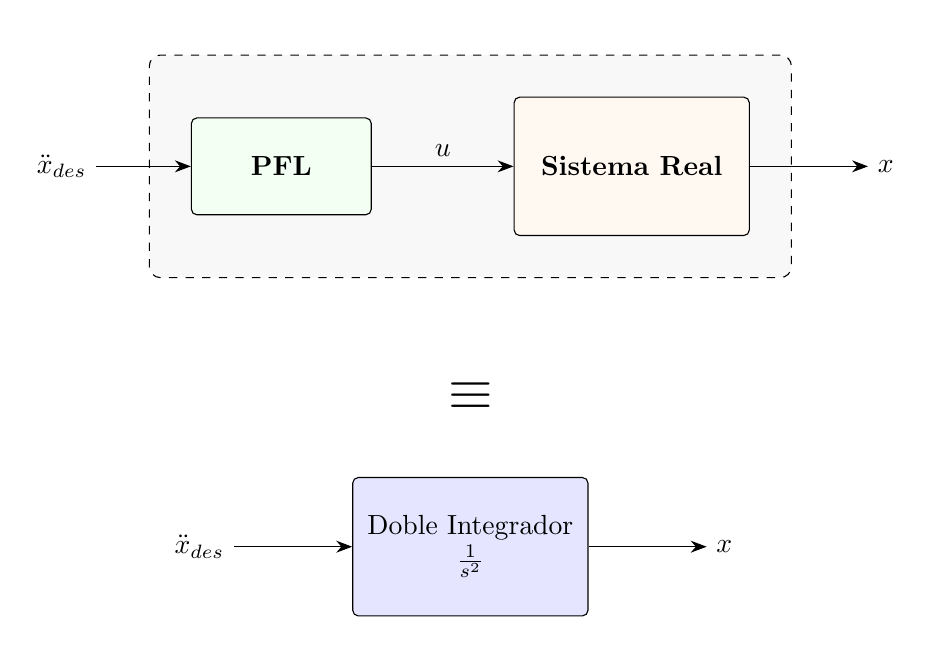
\begin{tikzpicture}[
		% Estilo calcado de tu diagrama principal
		block/.style = {draw, rectangle, minimum height=3.5em, minimum width=6.5em, align=center, rounded corners=2pt},
		% Estilo para la caja envolvente de la equivalencia
		env_box/.style={draw, dashed, rounded corners=4pt, inner sep=15pt, fill=gray!10, fill opacity=0.5},
		node distance=1.5cm,
		>={Stealth[scale=1.2]}
		]
		
		% --- PARTE SUPERIOR: Sistema Real con PFL ---
		\node (in1) {$\ddot{x}_{des}$};
		\node [block, right=1.2cm of in1, fill=green!5] (pfl) {\textbf{PFL}};
		\node [block, right=1.8cm of pfl, fill=orange!5, minimum height=5em, minimum width=8.5em] (planta) {\textbf{Sistema Real}}; % Mismo tamaño que en tu diagrama
		\node [right=1.5cm of planta] (out1) {$x$};
		
		\draw [->] (in1) -- (pfl);
		\draw [->] (pfl) -- node[above] {$u$} (planta);
		\draw [->] (planta) -- (out1);
		
		% --- CAPA DE FONDO (Caja de equivalencia) ---
		\begin{scope}[on background layer]
			\node [env_box, fit=(pfl) (planta)] (equiv) {};
			\node [above=0.1cm of equiv.north] {};
		\end{scope}
		
		% --- SÍMBOLO DE EQUIVALENCIA ---
		\node [below=1.2cm of equiv] (eq_sign) {\huge $\equiv$};
		
		% --- PARTE INFERIOR: Modelo Equivalente (Doble Integrador) ---
		\node [below=1.5cm of eq_sign] (centro_modelo) {}; 
		
		\node [block, fill=blue!10, minimum width=8.5em, minimum height=5em] at (centro_modelo) (modelo) {Doble Integrador \\ $\frac{1}{s^2}$}; % Ajustado para que visualmente pese parecido al sistema real
		\node [left=1.5cm of modelo] (in2) {$\ddot{x}_{des}$};
		\node [right=1.5cm of modelo] (out2) {$x$};
		
		\draw [->] (in2) -- (modelo);
		\draw [->] (modelo) -- (out2);
		
	\end{tikzpicture}
\end{document}